\bookchapter{الفصل 42: مشهد النماذج اللغوية الكبيرة والتطبيق العملي لواجهات API}

\chapterintro{تناوبت الفصول السابقة «كيف تتعاون مع الذكاء الاصطناعي»، أما هذا الفصل فيعالج سؤالًا أكثر أساسية: «أي ذكاء اصطناعي تستخدم؟ وكيف تستخدمه؟». صار مشهد النماذج اللغوية الكبيرة في أغسطس 2026 بالغ الثراء — فعلى الساحة الدولية تتنافس ثلاث قوى كبرى هي GPT وClaude وGemini، وفي الصين تزدهر نماذج DeepSeek وتونغ يي تشيون وِن وGLM وKimi ودو باو. ولكل نموذج شخصيته وميزته الخاصة: الاختيار الصحيح يقلل الجهد ويضاعف النتيجة، والاختيار الخاطئ يضاعف الجهد ويقلل النتيجة. لن يعرّفك هذا الفصل بهذه النماذج فحسب، بل سيعلمك أيضًا كيف تربطها بتطبيقك عبر API، وكيف تختار خطة التوكنات (Token Plan) المناسبة حسب احتياجك.}

\booksection{أولًا: النماذج اللغوية الكبيرة الدولية الرائدة: مشهد القوى الثلاث}

شكّل سوق النماذج اللغوية الكبيرة الدولي في أغسطس 2026 مشهدًا تقوده ثلاث قوى: OpenAI (سلسلة GPT) وAnthropic (سلسلة Claude) وGoogle (سلسلة Gemini). ولكل شركة سماتها الواضحة — فلنتعرف عليها واحدة تلو الأخرى.

\booksubsection{سلسلة GPT-5.6 من OpenAI: المحارب الشامل المتوازن}

OpenAI هي الشركة التي أطلقت موجة النماذج اللغوية الكبيرة، ولا تزال سلسلة GPT حتى اليوم النماذج الأوسع استخدامًا عالميًا. واعتمدت سلسلة GPT-5.6 الصادرة في يوليو 2026 استراتيجية ثلاثة مستويات: النموذج الرائد GPT-5.6 Sol لاحتياجات الاستدلال المتقدمة، والنموذج المتوازن GPT-5.6 Terra للتطوير اليومي، والنموذج الخفيف GPT-5.6 Luna للسيناريوهات عالية التزامن ومنخفضة التكلفة. وتتشارك النماذج الثلاثة نافذة سياق تبلغ 1.05 مليون توكن، وجميعها تدعم إدخال الصور واستدعاء الدوال والمخرجات المهيكلة.

\begin{center}
\begin{tabularx}{\linewidth}{|X|X|X|X|X|}
\hline
\textbf{الطراز} & \textbf{الفئة} & \textbf{الإدخال (لكل مليون توكن)} & \textbf{الإخراج (لكل مليون توكن)} & \textbf{نافذة السياق} \tabularnewline
\hline
GPT-5.6 Sol & رائد للاستدلال & 5.00 دولار أمريكي (نحو 36 يوانًا) & 30.00 دولار أمريكي (نحو 217 يوانًا) & 1.05 مليون توكن \tabularnewline
GPT-5.6 Terra & متوازن للاستخدام اليومي & 2.50 دولار أمريكي (نحو 18 يوانًا) & 15.00 دولار أمريكي (نحو 109 يوانات) & 1.05 مليون توكن \tabularnewline
GPT-5.6 Luna & خفيف ومنخفض التكلفة & 1.00 دولار أمريكي (نحو 7 يوانات) & 6.00 دولار أمريكي (نحو 44 يوانًا) & 1.05 مليون توكن \tabularnewline
\hline
\end{tabularx}
\end{center}

\begin{center}\small\color{gray}أسعار سلسلة GPT-5.6 من OpenAI (أغسطس 2026)\end{center}

تكمن الميزة الجوهرية لسلسلة GPT في «التوازن» — استدلال وبرمجة وكتابة وتعدد وسائط دون نقاط ضعف واضحة. وتضاف إلى ذلك منظومة الإضافات الضخمة لدى OpenAI ومجتمع المطورين، وهي الأكثر اكتمالًا في الوثائق المتوافقة وسلاسل الأدوات. وفي السيناريوهات التي «لا تعرف فيها ماذا تختار»، فإن GPT هي الإجابة الافتراضية التي «لا تخيب وإن اخترتها وأنت مغمض العينين». لكن نقاط ضعفها: الوصول إليها من داخل الصين يتطلب شبكة خاصة، وأداؤها في التعبير بالصينية يحمل أحيانًا «طبعًا مترجمًا»، وأسعار API فيها متوسطة إلى مرتفعة.

\textbf{خبر سار}\par

أعلنت OpenAI في أغسطس 2026 ترقية النموذج الافتراضي للمستخدمين المجانيين إلى GPT-5.6 Luna، وفتح الدردشة النصية بلا حدود. هذا يعني أنه يمكنك تجربة القدرات الأساسية لـ GPT دون أي تكلفة، ولن تحتاج إلى الدفع إلا عند الحاجة إلى استدلال أقوى أو استدعاء عبر API.

\booksubsection{سلسلة Claude من Anthropic: قمة البرمجة والدقة}

إذا كانت GPT لاعبة شاملة، فإن Claude هو «القمة» في مجال البرمجة. فسلسلة Claude من Anthropic تتقدم بفارق ساحق ومستمر في اختبار SWE-bench (المعيار المرجعي لهندسة البرمجيات)، وتحتل المرتبة الأولى صناعيًا في جودة توليد الشيفرة والقدرة على تنفيذ المشاريع بمستوى هندسي. والأثمن من ذلك أن معدل الهلوسة في Claude (احتمال توليد معلومات زائفة) هو الأدنى على الإطلاق بنحو 1\% فقط — وهذا يجعله مناسبًا بشكل خاص للسيناريوهات عالية الدقة مثل الأوساط الأكاديمية والشؤون القانونية.

ورقة Claude الرابحة الأخرى هي السياق فائق الطول: فهو يدعم نافذة سياق تبلغ مليون توكن، ويستطيع «قراءة» عقد من مئات الصفحات أو مكتبة شيفرة كاملة دفعة واحدة دون تفويت التفاصيل. وهذا أمر بالغ الصعوبة في السيناريوهات مثل إعادة هيكلة الشيفرة وتحليل المستندات الطويلة. وClaude Code بوصفه أداة برمجة بالذكاء الاصطناعي في الطرفية بلغت إيراداته السنوية 2.5 مليار دولار بحلول منتصف 2026 — وهو أقوى دليل على الاعتراف الواسع بقدرات Claude البرمجية.

\begin{center}
\begin{tabularx}{\linewidth}{|X|X|X|X|X|}
\hline
\textbf{الطراز} & \textbf{الفئة} & \textbf{الإدخال (لكل مليون توكن)} & \textbf{الإخراج (لكل مليون توكن)} & \textbf{نافذة السياق} \tabularnewline
\hline
Claude Fable 5 & الطراز الرائد & 10.00 دولار أمريكي (نحو 72 يوانًا) & 50.00 دولار أمريكي (نحو 362 يوانًا) & مليون توكن \tabularnewline
Claude Opus 4.8 & الطراز الاحترافي & 5.00 دولار أمريكي (نحو 36 يوانًا) & 25.00 دولار أمريكي (نحو 181 يوانًا) & مليون توكن \tabularnewline
Claude Sonnet 5 & طراز القيمة مقابل السعر & 2.00 دولار أمريكي (نحو 14 يوانًا) & 10.00 دولار أمريكي (نحو 72 يوانًا) & مليون توكن \tabularnewline
\hline
\end{tabularx}
\end{center}

\begin{center}\small\color{gray}أسعار سلسلة Claude من Anthropic (أغسطس 2026، وسعر Sonnet 5 مخفَّض)\end{center}

نقطة ضعف Claude هي السعر — فسعر الإخراج لدى Fable 5 هو الأعلى بين جميع النماذج، إذ يبلغ 50 دولارًا لكل مليون توكن. كما أن قدراته في تعدد الوسائط (فهم الصور والفيديو) ضعيفة نسبيًا. أما للمطورين الأفراد محدودي الميزانية، فإن Sonnet 5 خلال فترة الخصم يقدم قيمة استثنائية مقابل السعر.

\booksubsection{سلسلة Gemini من Google: ملك تعدد الوسائط}

وصلت سلسلة Gemini من Google بحلول 2026 إلى الإصدار 3.1 Pro. وأقوى ورقة لدى Gemini هي تعدد الوسائط الأصيل — تحليل دقيق للصور والنصوص، وتعرف بلا أخطاء على الجداول عبر OCR، واستخراج فعال لإطارات الفيديو، مع دعم التحليل المتعمق للصوت والفيديو. وهو مرتبط بعمق بمنظومة Google (البحث والبريد والخدمات السحابية)، ويتميز في استرجاع المعلومات في الوقت الفعلي والفهم عبر الوسائط. كما يدعم Gemini إدخال سياق فائق الطول يبلغ مليوني توكن، وهو النموذج صاحب أكبر نافذة سياق حتى الآن.

تموضع Gemini هو «الخيار الأول لسيناريوهات الاستدلال العلمي وتعدد الوسائط». إذا كان مشروعك يتضمن تحليلًا مكثفًا للصور أو فهم فيديو أو حسابات علمية، فلن يجد Gemini شبه منافس. لكنه يقل قليلًا عن Claude في توليد الشيفرة النصية الصرفة، كما أن تعبيره باللغة الصينية ليس بسلاسة النماذج الصينية.

\begin{center}
\begin{tabularx}{\linewidth}{|X|X|X|X|}
\hline
\textbf{بند المقارنة} & \textbf{GPT-5.6} & \textbf{Claude Fable 5} & \textbf{Gemini 3.1 Pro} \tabularnewline
\hline
الدرجة الإجمالية & 94.8 & 95.0 & 92.1 \tabularnewline
القدرة البرمجية (SWE-bench) & 74.9\% & 64.3\% (Pro) & متوسط \tabularnewline
نافذة السياق & 1.05 مليون توكن & مليون توكن & مليونا توكن \tabularnewline
قدرات تعدد الوسائط & متوازنة & أضعف نسبيًا & الأقوى \tabularnewline
معدل الهلوسة & منخفض نسبيًا & الأدنى (نحو 1\%) & منخفض نسبيًا \tabularnewline
الإتاحة داخل الصين & تتطلب شبكة خاصة & تتطلب شبكة خاصة & تتطلب شبكة خاصة \tabularnewline
منظومة API & الأكثر اكتمالًا & في طور النمو & مرتبط بمنظومة Google \tabularnewline
\hline
\end{tabularx}
\end{center}

\begin{center}\small\color{gray}مقارنة أفقية بين النماذج الدولية الثلاثة الكبرى (أغسطس 2026)\end{center}

\begin{tcbwarn}{تنبيه: العوائق الواقعية للاستخدام داخل الصين}
بالنسبة للمطورين داخل الصين، يتمثل العائق الأساسي أمام GPT وClaude وGemini في الوصول عبر الشبكة. ورغم إمكانية استخدامها بشكل غير مباشر عبر وسطاء Azure أو منصات تجميع API وغيرها، فإن الاستقرار والامتثال أمران ينبغي تقييمهما بنفسك. وإذا كان مشروعك يفرض متطلبات صارمة لأمن البيانات، فننصح بالنظر أولًا في النماذج الصينية.

\end{tcbwarn}

\booksection{ثانيًا: النماذج اللغوية الكبيرة الصينية الرائدة: ازدهار متعدد الألوان}

تحولت النماذج اللغوية الكبيرة الصينية في 2026 من «طاردة» إلى «منافسة في الصف الأول»، بل حققت «الصدارة» في بعض المجالات. وعلى خلاف جدل «الغلاف الخارجي» في 2023، أصبحت النماذج الصينية الرائدة في 2026 منافسة للنماذج الدولية من الطراز الأول في الاستدلال المنطقي وتوليد الشيفرة وفهم اللغة الصينية، وقد تقلصت الفجوة إلى ما دون 5\%. والأهم أن النماذج الصينية تتمتع بمزايا يصعب تعويضها في السيناريوهات الصينية والتكلفة والنشر المطابق للأنظمة.

\booksubsection{DeepSeek V4: ملك القيمة مقابل السعر}

DeepSeek (شن دو تشيو سو) ظاهرة بارزة بين النماذج اللغوية الكبيرة الصينية. ففي مطلع 2025 صدمت DeepSeek-V3 السوق بتموضع «أرخص من GPT بعُشر السعر وبالقدرة نفسها»، وسمتها الأوساط الصناعية «خط الإسقاط للنماذج اللغوية العامة» — فما هو أرخص منها ليس بجودتها، وما هو أغلى منها لا يضاهي وفرة إمكانياتها. وبحلول أغسطس 2026 صدرت النسخة الرسمية DeepSeek V4-Pro: بنية MoE بـ 1.6 تريليون معامل مع تنشيط نحو 49 مليار منها، ودعم سياق بلا فقدان يبلغ مليون توكن، وتُعد قيمتها مقابل السعر في البرمجة على نطاق واسع القمة عالميًا.

قفزت قدرات الوكيل (Agent) في DeepSeek V4 قفزة كبيرة — إذ ارتفع معيار DeepSWE من 12.8 إلى 62.7 (+390\%)، وNL2Repo من 38.5 إلى 61.5. وأضاف الـ API دعم البروتوكولين معًا: Responses API وAnthropic API، وهو متوافق الآن مع أدوات البرمجة الرئيسية مثل Codex وClaude Code. هذا يعني أنه يمكنك استخدام API الخاص بـ DeepSeek بدلًا من API الخاص بـ Claude داخل Claude Code — بانخفاض التكلفة أضعافًا وبخبرة شبه مطابقة.

\begin{center}
\begin{tabularx}{\linewidth}{|X|X|X|X|X|}
\hline
\textbf{الطراز} & \textbf{الفئة} & \textbf{الإدخال (لكل مليون توكن)} & \textbf{الإخراج (لكل مليون توكن)} & \textbf{نافذة السياق} \tabularnewline
\hline
DeepSeek V4 Pro & رائد للاستدلال & 3 يوانات (نحو 0.43 دولار أمريكي) & 6 يوانات (نحو 0.87 دولار أمريكي) & مليون توكن \tabularnewline
DeepSeek V4 Flash & خفيف وسريع & يوان واحد (نحو 0.14 دولار أمريكي) & يوانان (نحو 0.28 دولار أمريكي) & مليون توكن \tabularnewline
\hline
\end{tabularx}
\end{center}

\begin{center}\small\color{gray}أسعار سلسلة DeepSeek V4 (أغسطس 2026، أسعار ترويجية)\end{center}

مقارنة الأسعار: مقابل مليون توكن إدخال + مليون توكن إخراج، تنفق DeepSeek V4 Flash نحو 0.42 دولار، وGPT-5.6 Sol نحو 35 دولارًا، وClaude Fable 5 نحو 60 دولارًا. فارق يصل إلى 80-140 ضعفًا.

\textbf{تحذير من الفخ: أسعار DeepSeek على وشك الارتفاع}\par

أعلنت DeepSeek رسميًا في 6 أغسطس 2026 عن «خطط لرفع أسعار API بشكل كبير قريبًا»، وقد لا تدوم الأسعار الترويجية طويلًا. وتشير شائعات في بعض وسائل الإعلام إلى أن الارتفاع قد يبلغ 30 ضعفًا، وحتى 14 أغسطس لم تعلن الشركة بعد عن خطة التسعير النهائية. فضلًا عن أن النسخة الرسمية من DeepSeek V4 أدخلت آلية تسعير حسب الذروة — إذ يتضاعف سعر الاستدعاء مباشرة في أوقات الذروة. ننصح بمتابعة الإعلانات الرسمية للحصول على أحدث الأسعار.

\booksubsection{Qwen3.7 Max من تونغ يي تشيون وِن: الخيار المؤسسي من Alibaba Cloud}

تعتمد سلسلة تونغ يي تشيون وِن (Qwen) من Alibaba Cloud على منظومة Alibaba Cloud، فتتمتع بميزة فطرية في النشر على مستوى المؤسسات. ونموذج Qwen3.7 Max الصادر في يوليو 2026 هو الرائد الحالي: نموذج كثيف بـ 235 مليار معامل، وسياق أصلي يبلغ 256K قابل للتوسيع حتى مليون. وتكمن المزايا الجوهرية لـ Qwen في: نضج منظومته مفتوحة المصدر (سلسلة كاملة مفتوحة المصدر من 7B إلى 235B)، ودقته في فهم السيناريوهات الصينية، وتكامله العميق مع بنية Alibaba Cloud التحتية.

\begin{center}
\begin{tabularx}{\linewidth}{|X|X|X|}
\hline
\textbf{الطراز} & \textbf{سعر الإخراج (لكل مليون توكن)} & \textbf{السيناريوهات المناسبة} \tabularnewline
\hline
qwen-turbo & 0.6 يوان & أسئلة وأجوبة مبسطة، وتصنيف نصوص، وتزامن عالٍ \tabularnewline
qwen-long & 2.0 يوان & معالجة سياق فائق الطول يبلغ 10 ملايين توكن \tabularnewline
qwen3.7-flash & 7.2 يوان & المحادثات العامة وتوليد المحتوى \tabularnewline
qwen3.7-plus & 12.0 يوانًا & تعدد الوسائط (صور + فيديو)، والإبداع باللغة الصينية \tabularnewline
qwen3.7-max & 36.0 يوانًا & القدرات الصينية الرائدة، والمهام المعقدة \tabularnewline
\hline
\end{tabularx}
\end{center}

\begin{center}\small\color{gray}التسعير المتدرج لسلسلة Qwen من تونغ يي تشيون وِن (أغسطس 2026)\end{center}

يعتمد تسعير Qwen استراتيجية متدرجة — من qwen-turbo منخفض التكلفة جدًا (إخراج 0.6 يوان لكل مليون توكن) إلى الرائد qwen3.7-max (إخراج 36 يوانًا لكل مليون توكن)، ليغطي احتياجات جميع السيناريوهات من الأسئلة الخفيفة إلى الاستدلال المعقد. وبالنسبة للشركات التي تستخدم Alibaba Cloud بالفعل، يُعد Qwen خيار التكامل الأسهل.

\booksubsection{GLM-5.1 من Zhipu: الأول بين النماذج الصينية في SWE-bench}

تألقت سلسلة GLM من Zhipu AI في 2026. إذ حقق GLM-5.1 المركز الأول بين النماذج الصينية في SWE-bench: بنية هجينة MoE بـ 744 مليار معامل، ودعم سياق يبلغ مليون توكن. ويتميز بفهمه الدقيق للدلالات الصينية، ودعمه للنشر الخاص المطابق للأنظمة داخل الصين — وهو أمر بالغ الأهمية لسيناريوهات التمويل والحكومة ذات المتطلبات الصارمة لأمن البيانات. أما تسعير GLM-5.1 فهو 6 يوانات للإدخال و24 يوانًا للإخراج لكل مليون توكن، وهو في المستوى المتوسط بين النماذج الصينية.

\booksubsection{Kimi K3: ملك النصوص فائقة الطول}

تشتهر سلسلة Kimi من شركة Moonshot AI بقدرتها على معالجة النصوص فائقة الطول. ونموذج Kimi K3 الصادر في يوليو 2026 يبلغ حجمه 2.8 تريليون معامل، ودخل الصف الأول عالميًا في تقييمات مهام معقدة متعددة. والسيناريو الجوهري لـ Kimi هو تحليل مكتبات الشيفرة الطويلة والاسترجاع المعزز للمستندات الطويلة — فهو يستطيع معالجة نص كتاب كامل أو شيفرة مشروع بأكمله، ويقدم أداءً متميزًا في مهام الاسترجاع من نوع «إبرة في كومة قش». وتسعيرة Kimi مرتفعة نسبيًا (نحو 12-20 يوانًا للإخراج لكل مليون توكن)، لكن لا أحد يضاهي قيمته مقابل السعر في سيناريوهات النصوص الطويلة.

\booksubsection{دو باو Doubao: اللاعب الشامل من ByteDance}

قدمت سلسلة دو باو (Doubao) من ByteDance أداءً مستقرًا في 2026. ونموذج Doubao Seed 2.1 Pro هو النموذج الرائد من Volcano Engine بسياق 256K، ويقدم أداءً إجماليًا مستقرًا في الاختبارات الفعلية مع تجربة بارزة في السيناريوهات الصينية. وتكمن مزايا دو باو في: توكنات مجانية كبيرة تُمنح فور التسجيل، وتكامل مكتمل مع منظومة Volcano Engine، وتسعير في أحد أدنى المستويات داخل الصين. وللمبتدئين الراغبين في تجربة البرمجة بالذكاء الاصطناعي سريعًا، يُعد دو باو خيارًا للبدء دون أي عتبة.

\begin{center}
\begin{tabularx}{\linewidth}{|X|X|X|X|X|X|}
\hline
\textbf{بند المقارنة} & \textbf{DeepSeek V4} & \textbf{Qwen3.7 Max} & \textbf{GLM-5.1} & \textbf{Kimi K3} & \textbf{دو باو 2.1 Pro} \tabularnewline
\hline
الدرجة الإجمالية & 87.5 & 89.7 & 90.5 & 88+ & 85+ \tabularnewline
القدرة البرمجية & قوية للغاية & قوي & الأول بين النماذج الصينية في SWE & قوي & فوق المتوسط \tabularnewline
فهم اللغة الصينية & ممتاز & ممتاز & دقيق & ممتاز & ممتاز \tabularnewline
نافذة السياق & مليون & 256K-1M & مليون & فائق الطول & 256K \tabularnewline
سعر الإخراج (يوان/مليون) & 6 & 36 & 24 & 12-20 & 30 \tabularnewline
مفتوح المصدر & رخصة MIT & السلسلة كلها مفتوحة المصدر & مفتوح المصدر جزئيًا & مغلق المصدر & مغلق المصدر \tabularnewline
النشر الخاص & مدعوم & مدعوم & مدعوم & غير مدعوم & غير مدعوم \tabularnewline
\hline
\end{tabularx}
\end{center}

\begin{center}\small\color{gray}مقارنة أفقية بين النماذج الصينية الخمسة الكبرى (أغسطس 2026)\end{center}

أحد الاتجاهات المهمة هو أن «الإحساس بفجوة الأجيال» بين النماذج الصينية وGPT/Claude قد زال. ففي الاستدلال المنطقي ومسابقات الرياضيات، يبقى الفارق بين النماذج الصينية الرائدة وGPT-5 في خانة الأرقام المفردة غالبًا. وفي التفكير المعماري المنهجي والاستدلال الهندسي المعقد، لا يزال Claude متقدمًا — إذ يقدم حلولًا معمارية أكثر «روحًا وإبداعًا»، بينما تبدو النماذج الصينية أحيانًا «جمادة تتبع القوالب». لكن في السيناريوهات الصينية وضبط التكلفة والنشر المطابق للأنظمة، تتمتع النماذج الصينية بأفضلية ساحقة.

\begin{center}
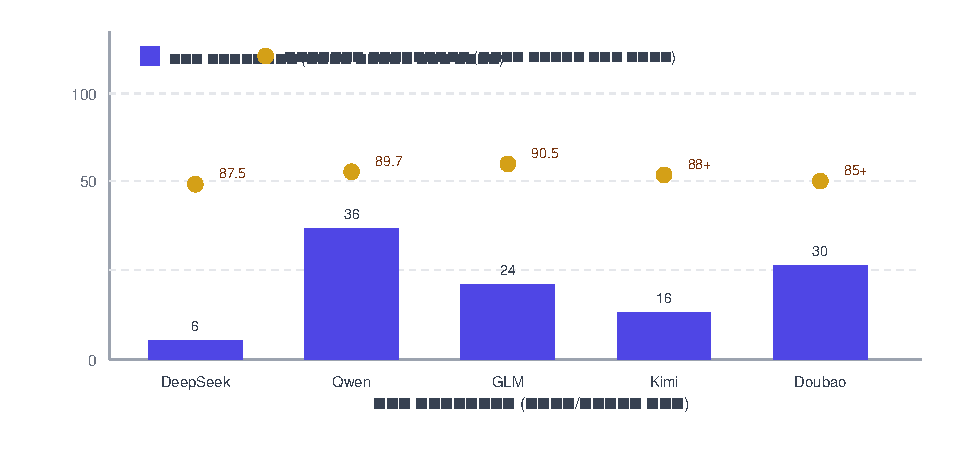
\includegraphics[width=0.92\linewidth]{figures/fig-di-si-shi-er-zhang-1}
\\[2pt]\small الشكل 4: مقارنة الأسعار والأداء بين النماذج الخمسة (كلما انخفض السعر كان أفضل، وكلما ارتفعت الدرجة كان أفضل)
\end{center}

\booksection{ثالثًا: إطار اتخاذ قرار اختيار النموذج}

بعد التعرف على خصائص كل نموذج، كيف تختار النموذج المناسب لمشروعك؟ نقدم لك هنا «طريقة الأسئلة الأربعة لاتخاذ القرار» — أجب عن أربعة أسئلة فتحدد النموذج الأنسب لك.

هل مشروعك يُنشر داخل الصين أم دوليًا؟

داخل الصين اختر نماذج محلية

|

دوليًا يمكن اختيار نماذج أجنبية

هل المهمة الأساسية برمجة أم شيء آخر؟

برمجة Claude أو DeepSeek

|

شيء آخر تابع التقييم

تحتاج سياقًا طويلًا جدًا (>500 ألف رمز)؟

نعم Gemini أو Kimi

|

لا حاجة تابع التقييم

هل الميزانية ضيقة؟

ضيقة DeepSeek أو Qwen-turbo

|

ليست ضيقة GPT-5.6 أو Claude

\begin{center}\small\color{gray}الشكل 5: طريقة الأسئلة الأربعة لاختيار النموذج اللغوي الكبير\end{center}

\begin{tcbinfo}{نصيحة: استراتيجية الدمج}
هذه الطريقة ليست قاعدة جامدة — فكثير من السيناريوهات تتطلب استخدام عدة نماذج مجتمعة. ومن استراتيجيات الدمج الشائعة: استخدام DeepSeek أو Qwen للتطوير اليومي (تكلفة منخفضة وكفاءة في الصينية)، وClaude لتصميم البنية الحاسمة (استدلال قوي وهلوسة منخفضة)، وGemini لتحليل الوسائط المتعددة (معالجة الصور والفيديو). بدِّل النموذج حسب الحاجة بدلًا من «الاستمرار بنموذج واحد إلى الأبد».

\end{tcbinfo}

\booksection{رابعًا: مدخل إلى استدعاء API: ربط النماذج اللغوية الكبيرة من الصفر}

كثير من دروس البرمجة بالذكاء الاصطناعي تكتفي بتعليمك استخدام واجهة المحادثة، لكن «البرمجة بالذكاء الاصطناعي» الحقيقية — أي جعل تطبيقك يستدعي النموذج اللغوي الكبير — تتم عبر API. فالـ API (Application Programming Interface، واجهة برمجة التطبيقات) هي بروتوكول اتصال بين البرامج. وعبر API يمكن لشيفرة أن تستدعي قدرات النموذج اللغوي الكبير كما تستدعي دالة.

\booksubsection{ما هو التوكن (Token)}

قبل التعرف على API، لا بد أولًا من فهم مفهوم «التوكن» (Token). التوكن هي وحدة الحساب الأساسية في النماذج اللغوية الكبيرة، ويمكن اعتبارها «وحدة القراءة والكتابة لدى الذكاء الاصطناعي». التوكن الواحد يقابل تقريبًا: 0.75 كلمة إنجليزية (4 محارف)، أو 0.5-1 حرف صيني. ونص صيني من 1000 حرف يستهلك نحو 1500-2000 توكن.

التوكن ليس عدد الكلمات ولا عدد المحارف. تستخدم النماذج اللغوية الكبيرة مُقسِّمًا للكلمات (Tokenizer) متخصصًا لتقطيع النص إلى توكنات. وقد يختلف عدد توكنات الكلمة الواحدة بين نموذج وآخر — فمثلًا قد تكون كلمة «الذكاء الاصطناعي» بالصينية 3 توكنات في GPT وتوكنين في DeepSeek. وتعيد API معظم النماذج عدد التوكنات المستهلكة فعليًا، ويمكنك الاطلاع عليه في استجابة الـ API.

\begin{tcbinfo}{تقدير سريع لتكلفة التوكنات}
مليون حرف صيني يقابل نحو 1.5 مليون توكن. بمعالجة مليون حرف إدخال + مليون حرف إخراج باستخدام DeepSeek V4 Flash تبلغ التكلفة نحو 0.42 دولار (نحو 3 يوانات)، وباستخدام Claude Fable 5 للكمية نفسها تبلغ نحو 60 دولارًا (نحو 434 يوانًا). لهذا فإن اختيار النموذج يؤثر مباشرة في تكلفة مشروعك.

\end{tcbinfo}

\booksubsection{الحصول على مفتاح API}

الخطوة الأولى لاستخدام API النماذج اللغوية الكبيرة هي الحصول على مفتاح API — سلسلة رموز تُستخدم للتحقق من الهوية. ولكل مزود نموذج منصته الخاصة لـ API، وتحتاج إلى تسجيل حساب وإنشاء المفتاح. وإليك بوابات منصات API للنماذج الرئيسية وخطوات الحصول عليها:

\begin{center}
\begin{tabularx}{\linewidth}{|X|X|X|X|}
\hline
\textbf{النموذج} & \textbf{منصة API} & \textbf{خطوات الحصول} & \textbf{الحصة المجانية} \tabularnewline
\hline
DeepSeek & platform.deepseek.com & التسجيل التحقق من الهوية إنشاء مفتاح API & حصة تُمنح للمستخدمين الجدد \tabularnewline
تونغ يي تشيون وِن (Qwen) & bailian.aliyun.com (منصة Bailian) & تسجيل الدخول بحساب Alibaba Cloud تفعيل الخدمة إنشاء المفتاح & تجربة مجانية للمستخدمين الجدد \tabularnewline
Zhipu GLM & open.bigmodel.cn & التسجيل التحقق من الهوية إنشاء مفتاح API & حصة تُمنح للمستخدمين الجدد \tabularnewline
Kimi & platform.moonshot.cn & التسجيل التحقق من الهوية إنشاء مفتاح API & حصة مجانية محدودة \tabularnewline
دو باو (Doubao) & volcengine.com (Volcano Engine) & التسجيل تفعيل خدمة Ark إنشاء مفتاح API & توكنات مجانية كثيرة عند التسجيل \tabularnewline
OpenAI GPT & platform.openai.com & التسجيل ربط بطاقة ائتمانية إنشاء مفتاح API & لا حصة مجانية (يتطلب الدفع) \tabularnewline
Anthropic Claude & console.anthropic.com & التسجيل ربط البطاقة إنشاء مفتاح API & حصة صغيرة للمستخدمين الجدد \tabularnewline
\hline
\end{tabularx}
\end{center}

\begin{center}\small\color{gray}منصات API للنماذج الرئيسية وطرق الحصول على المفتاح (أغسطس 2026)\end{center}

\textbf{تنبيه أمني: مفتاح API = كلمة مرور محفظتك}\par

مفتاح API يعادل كلمة مرور محفظتك — فأي شخص يحصل على المفتاح يستطيع استدعاء النموذج على حساب حصتك. لذلك: لا تكتب مفتاح API أبدًا داخل الشيفرة (أدره عبر متغيرات البيئة)؛ ولا ترفع شيفرة تحتوي المفتاح إلى مستودع Git عام أبدًا؛ ولا تشارك لقطات شاشة تظهر المفتاح على وسائل التواصل الاجتماعي أبدًا. وإذا تسرب المفتاح فاحذفه فورًا على المنصة وأنشئ مفتاحًا جديدًا.

\booksubsection{أول استدعاء لـ API}

بعد الحصول على مفتاح API، يمكنك استدعاء API النماذج اللغوية الكبيرة بأي لغة برمجة. وفيما يلي مثال بأبسط استدعاء ممكن باستخدام Python — إرسال رسالة إلى DeepSeek والحصول على الرد.

\begin{lstlisting}[language=Python]
# تثبيت الـ SDK: pip install openai
# DeepSeek متوافق مع صيغة OpenAI SDK، يمكن استخدامه مباشرة
from openai import OpenAI
import os

# 1. إنشاء العميل (يُقرأ مفتاح API من متغير البيئة)
client = OpenAI(
    api_key=os.environ.get("DEEPSEEK_API_KEY"),
    base_url="https://api.deepseek.com"
)

# 2. إرسال الطلب
response = client.chat.completions.create(
    model="deepseek-chat",  # تحديد النموذج
    messages=[
        {"role": "system", "content": "أنت مساعد برمجة بلغة بايثون."},
        {"role": "user", "content": "اكتب دالة ترتيب سريع."}
    ]
)

# 3. الحصول على الرد
print(response.choices[0].message.content)

# 4. عرض استهلاك الرموز
print(f"رموز الإدخال: {response.usage.prompt_tokens}")
print(f"رموز المخرجات: {response.usage.completion_tokens}")
print(f"إجمالي الرموز: {response.usage.total_tokens}")
\end{lstlisting}

المنطق الجوهري لهذه الشيفرة هو: إنشاء العميل (مع مفتاح API وعنوان النموذج) بناء قائمة الرسائل (system يحدد الدور، وuser هو مدخل المستخدم) إرسال الطلب الحصول على الرد. هذا النمط يصلح تقريبًا لكل النماذج المتوافقة مع صيغة OpenAI — يكفي تغيير api\_key وbase\_url لتبديل النموذج. ولهذا تختار كثير من النماذج الصينية التوافق مع صيغة OpenAI SDK: يستطيع المطور تبديل النموذج بتغيير سطرين فقط، فتكون تكلفة الانتقال بالغة الانخفاض.

فيما يلي فروق الشيفرة عند التبديل إلى نماذج أخرى — لاحظ أن التغيير لا يتجاوز سطرين:

\begin{lstlisting}[language=Python]
# DeepSeek
client = OpenAI(
    api_key=os.environ.get("DEEPSEEK_API_KEY"),
    base_url="https://api.deepseek.com"
)
# model="deepseek-chat"

# Qwen (منصة Bailian)
client = OpenAI(
    api_key=os.environ.get("DASHSCOPE_API_KEY"),
    base_url="https://dashscope.aliyuncs.com/compatible-mode/v1"
)
# model="qwen-plus"

# GLM من Zhipu
client = OpenAI(
    api_key=os.environ.get("GLM_API_KEY"),
    base_url="https://open.bigmodel.cn/api/paas/v4"
)
# model="glm-4"

# OpenAI GPT
client = OpenAI(
    api_key=os.environ.get("OPENAI_API_KEY"),
    # يكفي base_url الافتراضي
)
# model="gpt-5.6-terra"
\end{lstlisting}

\booksubsection{معالجة الاستجابة المتدفقة}

في التطبيقات الفعلية، لن ترغب عادةً في الانتظار حتى يكتب الذكاء الاصطناعي كل المحتوى قبل عرضه دفعة واحدة — فهذا يجعل المستخدم ينتظر طويلًا. وتتيح لك الاستجابة المتدفقة (Streaming) عرض النص حرفًا بحرف أثناء توليده من الذكاء الاصطناعي، مما يحسّن تجربة المستخدم بشكل كبير. فمثل الآلة الكاتبة، تظهر الحروف واحدة تلو الأخرى، وشعور المستخدم يختلف تمامًا.

\begin{lstlisting}[language=Python]
# استجابة متدفقة: إخراج كلمة بكلمة
stream = client.chat.completions.create(
    model="deepseek-chat",
    messages=[
        {"role": "user", "content": "اكتب درسًا عن خوارزمية الترتيب الفقاعي في بايثون"}
    ],
    stream=True  # تفعيل البث المتدفق
)

# استلام وطباعة على شكل كتل
for chunk in stream:
    if chunk.choices[0].delta.content is not None:
        print(chunk.choices[0].delta.content, end="", flush=True)
# سيظهر الناتج حرفًا حرفًا مثل آلة كاتبة
\end{lstlisting}

\booksection{خامسًا: دليل شراء باقات التوكنات (Token Plan)}

تقدم معظم مزودي النماذج طريقتين للحساب: الدفع حسب الاستعمال (Pay-as-you-go) والاشتراك بالباقات (Token Plan / Subscription). وفهم الفرق بين الطريقتين يمكن أن يساعدك على خفض تكلفة الاستخدام بشكل كبير.

\booksubsection{الدفع حسب الاستعمال مقابل الاشتراك بالباقات}

\begin{center}
\begin{tabularx}{\linewidth}{|X|X|X|}
\hline
\textbf{البعد} & \textbf{الدفع حسب الاستعمال (Pay-as-you-go)} & \textbf{الاشتراك بالباقات (Subscription)} \tabularnewline
\hline
طريقة الحساب & تدفع مقابل التوكنات التي تستخدمها & تدفع مبلغًا ثابتًا مسبقًا مقابل حصة \tabularnewline
السيناريوهات المناسبة & استخدام غير مستقر أو استدعاءات متقطعة & استخدام مستقر واستدعاءات كثيفة \tabularnewline
الميزة السعرية & السعر القياسي & أقل من الدفع حسب الاستعمال بنسبة 20\%-50\% \tabularnewline
المرونة & متاح في أي وقت دون أي التزام & تتطلب دفعًا مسبقًا، وقد تنتهي صلاحية الحصة غير المستخدمة \tabularnewline
معالجة تجاوز الحصة & تحويل تلقائي إلى الدفع حسب الاستعمال & بعد تجاوز الحصة يتحول إلى الدفع حسب الاستعمال \tabularnewline
المنصات الممثلة & منصات API الرسمية لكل نموذج & OpenAI Plus/Pro, Claude Pro, Cursor Pro \tabularnewline
\hline
\end{tabularx}
\end{center}

\begin{center}\small\color{gray}مقارنة بين طريقتي الحساب\end{center}

للمبتدئين، ننصح بالبدء بالدفع حسب الاستعمال — فلا حاجة إلى دفع مسبق، وتدفع ما تستخدمه فقط. وحين يستقر استهلاكك الشهري عند مستوى معين (مثلًا تجاوز 50 يوانًا شهريًا)، فكّر حينها في الانتقال إلى الاشتراك بالباقات للحصول على سعر وحدة أقل.

\booksubsection{نظرة على باقات الاشتراك الرئيسية}

\begin{center}
\begin{tabularx}{\linewidth}{|X|X|X|X|}
\hline
\textbf{الباقة} & \textbf{الرسوم الشهرية} & \textbf{المحتوى المشمول} & \textbf{الفئة المناسبة} \tabularnewline
\hline
ChatGPT Free & مجانًا & دردشة نصية غير محدودة بنموذج GPT-5.6 Luna & تجربة للمبتدئين تمامًا \tabularnewline
ChatGPT Plus & 20 دولارًا أمريكيًا/شهريًا & GPT-5.6 Sol، وتوليد الصور، وتحليل البيانات، والوصول إلى الإضافات & المستخدمون متوسطو الاستخدام \tabularnewline
ChatGPT Pro & 200 دولار أمريكي/شهريًا & استخدام غير محدود لجميع النماذج، وأولوية الوصول إلى الميزات الجديدة & المستخدمون المحترفون كثيفو الاستخدام \tabularnewline
Claude Free & مجانًا & عدد محدود من محادثات Claude & تجربة للمبتدئين تمامًا \tabularnewline
Claude Pro & 20 دولارًا أمريكيًا/شهريًا & استخدام غير محدود لـ Claude، وأولوية الوصول إلى النماذج الجديدة & مطورو البرمجة \tabularnewline
Cursor Free & مجانًا & عدد محدود من إكمالات الذكاء الاصطناعي والمحادثات & تجربة للمبتدئين \tabularnewline
Cursor Pro & 20 دولارًا أمريكيًا/شهريًا & إكمال ذكاء اصطناعي غير محدود، و500 طلب متقدم شهريًا & المطورون في الاستخدام اليومي \tabularnewline
Cursor Business & 40 دولارًا أمريكيًا/شهريًا/للفرد & تعاون الفريق، ولوحة الإدارة، ووضع الخصوصية & الفرق والاستخدام الجماعي \tabularnewline
\hline
\end{tabularx}
\end{center}

\begin{center}\small\color{gray}باقات الاشتراك لأدوات الذكاء الاصطناعي الرئيسية (أغسطس 2026)\end{center}

تختلف خطط الاشتراك للنماذج الصينية قليلًا. فـ DeepSeek تعتمد أساسًا على الدفع حسب الاستعمال ولا تقدم باقات اشتراك شهرية — تُحمل رصيدًا ثم يُخصم وفق الاستهلاك الفعلي. وتقدم تونغ يي تشيون وِن حزم موارد مدفوعة مسبقًا على منصة Bailian (شراء كمية محددة من التوكنات بسعر مخفض). ولدى دو باو أيضًا خطط مدفوعة مسبقًا مشابهة على Volcano Engine. وبالنسبة للمطورين داخل الصين، فإن التوليفة الأكثر اقتصادية عادة هي: الدفع حسب الاستعمال لدى DeepSeek (للتطوير اليومي) + الحصة المجانية من دو باو (للتجربة والاختبار).

\booksubsection{منصات تجميع API}

إذا احتجت إلى استخدام عدة نماذج في آن واحد، فمنصات تجميع API خيار مريح. تقدم منصة التجميع مفتاح API واحدًا موحدًا تستطيع به استدعاء عشرات النماذج حول العالم دون الحاجة إلى التسجيل في كل منصة على حدة.

\begin{center}
\begin{tabularx}{\linewidth}{|X|X|X|X|}
\hline
\textbf{المنصة} & \textbf{الخصائص} & \textbf{الميزة السعرية} & \textbf{السيناريوهات المناسبة} \tabularnewline
\hline
OpenRouter (openrouter.ai) & منصة تجميع خارجية، بمفتاح واحد تستدعي نماذج العالم & أسعار شفافة مع مقارنة فورية للأسعار & لمن يحتاج إلى التبديل المرن بين عدة نماذج أجنبية \tabularnewline
SiliconFlow (siliconflow.cn) & منصة تجميع صينية توفر واجهات API لنماذج صينية متعددة & أقل من الأسعار الرسمية بنسبة 20\%-30\% & مطورون داخل الصين، ومقارنة أسعار بين عدة نماذج \tabularnewline
Azure OpenAI (وكيل Microsoft) & واجهة OpenAI API عبر وكيل Microsoft Azure & خصم 50\% مع Batch API & استدعاءات OpenAI على مستوى المؤسسات، للمهام الدفعية غير المتزامنة الكبيرة \tabularnewline
Baidu Qianfan (qianfan.baidubce.com) & منصة بايدو السحابية للذكاء الاصطناعي، توفر نماذج مثل ERNIE & رصيد مجاني هدية للمستخدمين الجدد & مستخدمو منظومة بايدو \tabularnewline
\hline
\end{tabularx}
\end{center}

\begin{center}\small\color{gray}أبرز منصات تجميع واجهات API (أغسطس 2026)\end{center}

\textbf{تنبيه من الفخ: لا تشترِ “مفاتيح مشتركة”}\par

لا تشترِ ما يُعرف بـ“مفاتيح API المشتركة” من منصات مثل Taobao أو Xianyu — فهذه المفاتيح مجهولة المصدر غالباً، وقد يُحظر حسابها في أي لحظة، إضافة إلى مخاطر تسرب البيانات. احصل على مفاتيح API دائماً من المنصات الرسمية أو منصات التجميع النظامية.

\booksubsection{استراتيجيات تحسين التكلفة}

اختيار النموذج المناسب هو الخطوة الأولى فقط، و“كيف تستخدمه بتكلفة أقل” لا تقل أهمية. إليك عدة استراتيجيات لتحسين التكلفة أثبتت جدواها عملياً:

\begin{enumerate}
  \item استفد جيداً من إصابة التخزين المؤقت. توفر نماذج كثيرة ميزة "التخزين المؤقت" (Cache) — حين يتضمن طلبك محتوى سبقت معالجته (مثل موجه النظام)، يُحتسب هذا الجزء بسعر منخفض جداً. سعر إصابة التخزين المؤقت لدى DeepSeek لا يزيد عن 1/60 من السعر العادي. ضع موجه النظام الثابت في بداية قائمة الرسائل لتعظيم نسبة إصابة التخزين المؤقت.
  \item التوجيه المتدرج — استخدم النموذج الرخيص للمهام البسيطة والنموذج الغالي للمهام المعقدة. مثلاً استخدم DeepSeek V4 Flash لتصنيف النصوص (المخرجات بسعر 2 يوان لكل مليون Token)، واستخدم Claude لتصميم البنية (المخرجات بسعر 181 يواناً لكل مليون Token). نحو 80\% من استدعاءات المشروع الواحد يمكن إنجازها بالنماذج الرخيصة.
  \item حدد طول المخرجات. تُحتسب واجهات API حسب Token المخرجات، وكلما طالت المخرجات ارتفعت التكلفة. في الحالات التي لا تحتاج فيها إلى إسهاب، اضبط معامل max\_tokens لتحديد طول المخرجات وتجنب "إسهاب الذكاء الاصطناعي".
  \item استخدم Batch API للمهام غير الفورية. إذا كانت لديك مهام كثيرة لا تتطلب استجابة فورية (مثل وسم البيانات الدفعي أو تلخيص المستندات)، فإن استخدام Batch API يمنحك خصماً بنسبة 50\%. توفر OpenAI وAzure هذه الميزة معاً.
  \item راقب استهلاك Token. توفر معظم منصات API لوحة إحصاءات للاستخدام. راجع توزيع الاستهلاك دورياً وحدد الاستدعاءات الأكثر استهلاكاً للـToken لتحسينها بشكل موجه. تعديل صغير في الموجه (مثل تغيير "اشرح بالتفصيل" إلى "اشرح في 3 جمل") قد يوفر 50\% من الـToken.
\end{enumerate}

\begin{center}
\begin{tabularx}{\linewidth}{|X|X|X|X|}
\hline
\textbf{استراتيجية التحسين} & \textbf{نسبة التوفير} & \textbf{صعوبة التنفيذ} & \textbf{الوصف} \tabularnewline
\hline
إصابة التخزين المؤقت & تصل إلى 98\% & منخفض & ضع المحتوى الثابت في بداية الرسائل \tabularnewline
التوجيه المتدرج & 50\%-80\% & متوسط & استخدم النموذج الرخيص للمهام البسيطة \tabularnewline
تحديد طول المخرجات & 30\%-60\% & منخفض & اضبط معامل max\_tokens \tabularnewline
Batch API & 50\% & منخفض & استخدم المعالجة الدفعية للمهام غير الفورية \tabularnewline
تحسين الموجهات (Prompt) & 20\%-50\% & متوسط & اختصر الموجه وقلل الحشو \tabularnewline
\hline
\end{tabularx}
\end{center}

\begin{center}\small\color{gray}استراتيجيات تحسين التكلفة ونتائجها (أغسطس 2026)\end{center}

\booksection{سادساً: تطبيق عملي — دمج واجهة النموذج الكبير API في مشروعك}

لنختم هذا الفصل بتطبيق عملي متكامل — إنشاء “مولد ملخصات بالذكاء الاصطناعي”: يدخل المستخدم نصاً طويلاً، فيستدعي التطبيق واجهة النموذج الكبير API لتوليد الملخص. سيعرض هذا التطبيق الدورة الكاملة لاستدعاء API: إعداد البيئة، الاستدعاء، معالجة الأخطاء، والتحكم في التكلفة.

\begin{lstlisting}[language=Python]
# ai_summarizer.py - مولّد ملخصات بالذكاء الاصطناعي
import os
from openai import OpenAI

# 1. الإعداد (يُقرأ مفتاح API من متغير البيئة، ولا يُكتب في الكود أبدًا)
client = OpenAI(
    api_key=os.environ.get("DEEPSEEK_API_KEY"),
    base_url="https://api.deepseek.com"
)

def summarize(text: str, max_length: int = 200) -> dict:
    """يولّد ملخصًا للنص

    Args:
        text: النص الأصلي المراد تلخيصه
        max_length: الطول الأقصى للملخص (عدد الرموز)

    Returns:
        dict: يتضمن الملخص ومعلومات استهلاك الرموز
    """
    try:
        response = client.chat.completions.create(
            model="deepseek-chat",
            messages=[
                {
                    "role": "system",
                    "content": "أنت مولّد ملخصات."
                               "لخص نص المستخدم بلغة واضحة وموجزة."
                               "الملخص لا يتجاوز 3 جمل."
                },
                {
                    "role": "user",
                    "content": f"لخص النص التالي:\n\n{text}"
                }
            ],
            max_tokens=max_length,  # يحدد طول المخرجات
            temperature=0.3  # حرارة منخفضة = أكثر استقرارًا
        )

        return {
            "success": True,
            "summary": response.choices[0].message.content,
            "input_tokens": response.usage.prompt_tokens,
            "output_tokens": response.usage.completion_tokens,
            "total_tokens": response.usage.total_tokens
        }

    except Exception as e:
        return {
            "success": False,
            "error": str(e)
        }

# 2. مثال للاستخدام
if __name__ == "__main__":
    long_text = """
    (الصق نصًا طويلًا هنا...)
    """

    result = summarize(long_text)

    if result["success"]:
        print(f"الملخص: {result['summary']}")
        print(f"الرموز المستهلكة: {result['total_tokens']}")
        # تقدير التكلفة: DeepSeek V4 Flash
        cost = result['total_tokens'] * 0.000004  # $\approx$ 0.4 سنت لكل 1000 رمز
        print(f"التكلفة التقديرية: {cost:.4f} يوان")
    else:
        print(f"حدث خطأ: {result['error']}")
\end{lstlisting}

يجسد هذا الكود عدة ممارسات مثلى لاستدعاء API: يُقرأ مفتاح API من متغيرات البيئة ولا يُكتب مطلقاً داخل الكود؛ للدالة توثيق واضح وتلميحات أنواع؛ ضُبط max\_tokens لتحديد طول المخرجات؛ وعينت temperature على قيمة منخفضة (0.3) لمخرجات أكثر استقراراً؛ توجد معالجة أخطاء كاملة؛ وتُعاد معلومات استهلاك Token لتتبع التكلفة. وعندما تستعين بالذكاء الاصطناعي لكتابة هذا الكود، أبلغه بهذه المتطلبات — فهو قادر تماماً على تحقيقها لك.

الخلاصة النهائية لهذا الفصل: النماذج "ذخيرة" والمنهجية "تكتيك". اختيار الذخيرة الصحيحة يجعل المعركة أسهل، لكن بدون تكتيك جيد لن تربح الحرب ولو كانت الذخيرة ممتازة. بعد أن تعرفت على خصائص كل نموذج وطريقة استخدام الـ API، أصبح لديك "مستودع ذخيرة" وافر، أما كيف تخوض المعركة فيعتمد على منهجية التفكير التي تعلمتها في الفصول السابقة.

\begin{tcbpractice}{لنطبق عملياً: نفذ أول استدعاء API لك بنجاح}
سجل في منصة نماذج صينية (نوصي بـ DeepSeek أو Zhipu، وكلاهما يمنح رصيداً للمستخدمين الجدد)، وأنشئ مفتاح API، واكتبه في متغيرات بيئة النظام (وليس في الكود!)، ثم شغل كود “أول استدعاء API” أعلاه. في اللحظة التي ترى فيها رد الذكاء الاصطناعي مطبوعاً أمامك، تكون قد اجتزت الخط الفاصل بين “استخدام الذكاء الاصطناعي” و“بناء تطبيقات الذكاء الاصطناعي”.

\end{tcbpractice}

\begin{tcbsummary}{خلاصة الفصل}
\begin{itemize}
  \item الثلاثي الدولي الكبير: GPT-5.6 (متوازن وشامل)، Claude (قمة البرمجة ونسبة هلوسة 1\% فقط)، Gemini (ملك تعدد الوسائط وسياق يتسع لمليوني Token)
  \item الخماسي الصيني الكبير: DeepSeek V4 (ملك القيمة مقابل السعر، وانتبه لإعلانات رفع الأسعار)، Qwen3.7 (للمؤسسات)، GLM-5.1 (الأول محلياً في SWE)، Kimi K3 (النصوص فائقة الطول)، Doubao (مجاني للمبتدئين)
  \item طريقة القرار بالأسئلة الأربعة: أين النشر؟ برمجة أم غيرها؟ سياق فائق الطول؟ حساسية للميزانية؟
  \item Token وحدة الفوترة: الحرف الصيني الواحد يساوي نحو 1.5-2 Token، ومليون حرف صيني يساوي نحو 1.5 مليون Token
  \item مفتاح API = كلمة سر محفظتك: يُدار عبر متغيرات البيئة، ولا يُكتب في الكود مطلقاً ولا يُرفع إلى Git
  \item النماذج الصينية متوافقة عموماً مع OpenAI SDK: لتبديل النموذج يكفي تعديل سطرين هما api\_key وbase\_url
  \item خمس حيل للتوفير: إصابة التخزين المؤقت، التوجيه المتدرج، تحديد المخرجات، Batch API، مراقبة الاستهلاك
\end{itemize}

\end{tcbsummary}
